%%%%%%%%%%%%%%%%%%%%%%%%%%%%%%%%%%%%%%%%%%%%%%%%
% Öffnungsschilder: was gerade im FabLab stattfindet (eine Seite je Termin)
% CC-BY-SA 3.0, FAU FabLab
% Früher Hinweisschilder_divers/oeffnungsschilder.pdf (Illustrator), jetzt LaTeX.
%%%%%%%%%%%%%%%%%%%%%%%%%%%%%%%%%%%%%%%%%%%%%%%%
\documentclass[a4paper,landscape]{scrartcl}
\usepackage{fablab-aushang}
\Fabcube

% \Termin{Name}{Farbe}{Satz im Balken}
\newcommand{\Termin}[3]{%
  \SchildKopf[0.9]{Jetzt: \textbf{#1}}
  \Banner[#2]{\fontsize{1.3\SchildText}{1.5\SchildText}\selectfont #3}
  \vspace{0.6\SchildText}}

\begin{document}
\Schild

\Termin{OpenLab}{fcGruen}{Komm rein -- lern das Lab kennen!}
\begin{Spalte}[0.62\linewidth]
Während des OpenLabs kannst du:
\begin{itemize}
  \item Fragen stellen und das FabLab kennenlernen
  \item in Geräte eingewiesen werden
  \item an eigenen Projekten arbeiten
\end{itemize}
\end{Spalte}
\newpage

\Termin{SelfLab}{fcBlau}{Arbeite an deinen Projekten.}
\begin{Spalte}[0.62\linewidth]
Während des SelfLabs kannst du:
\begin{itemize}
  \item dich im Lab umschauen
  \item mit vorhandener Einweisung an eigenen Projekten arbeiten
\end{itemize}
\end{Spalte}
\newpage

\Termin{Workshop}{fcRot}{Leider nur mit Anmeldung.}
\begin{Spalte}[0.62\linewidth]
Komm doch ein anderes Mal wieder.

Unsere Öffnungszeiten findest du auf \texttt{fablab.fau.de/termine}

Wir freuen uns auf dich :)
\end{Spalte}
\newpage

\Termin{Arbeitstreffen}{fcBlau}{Hilf uns, das Lab zu verbessern.}
\begin{Spalte}[0.62\linewidth]
Während des Arbeitstreffens kannst du:
\begin{itemize}
  \item dich im Lab umschauen
  \item aktiv das FabLab mitgestalten
  \item unsere Betreuer kennenlernen
  \item erfahren, wie du selbst Betreuer wirst
\end{itemize}
\end{Spalte}
\newpage

\Termin{Aktiventreffen}{fcGruen}{Mach mit, sei dabei, werd aktiv!}
Das Treffen findet im Aquarium statt:\par
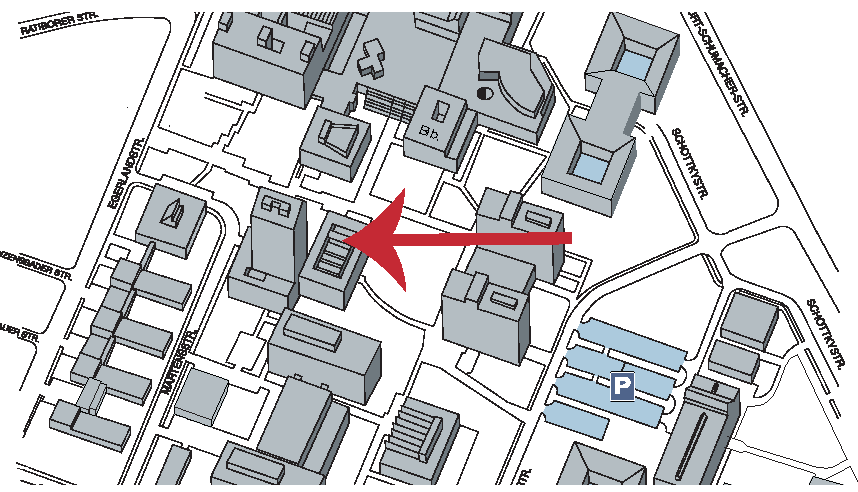
\includegraphics[height=0.44\textheight]{img/karte-aquarium.pdf}

\end{document}
